\documentclass[journal,12pt,twocolumn]{IEEEtran}
\usepackage{setspace}
\usepackage{gensymb}
\singlespacing
\usepackage[cmex10]{amsmath}

\usepackage{amsthm}
\usepackage{hyperref}
\hypersetup{
    colorlinks=true,
    linkcolor=blue,
    filecolor=magenta,      
    urlcolor=cyan,
}

\urlstyle{same}
\usepackage{mathrsfs}
\usepackage{txfonts}
\usepackage{stfloats}
\usepackage{bm}
\usepackage{cite}
\usepackage{cases}
\usepackage{subfig}

\usepackage{longtable}
\usepackage{multirow}

\usepackage{enumitem}
\usepackage{mathtools}
\usepackage{steinmetz}
\usepackage{tikz}
\usepackage{circuitikz}
\usepackage{verbatim}
\usepackage{tfrupee}
\usepackage[breaklinks=true]{hyperref}
\usepackage{graphicx}
\usepackage{tkz-euclide}

\usetikzlibrary{calc,math}
\usepackage{listings}
    \usepackage{color}                                            %%
    \usepackage{array}                                            %%
    \usepackage{longtable}                                        %%
    \usepackage{calc}                                             %%
    \usepackage{multirow}                                         %%
    \usepackage{hhline}                                           %%
    \usepackage{ifthen}                                           %%
    \usepackage{lscape}     
\usepackage{multicol}
\usepackage{chngcntr}
\usepackage{mdframed}
\DeclareMathOperator*{\Res}{Res}

\renewcommand\thesection{\arabic{section}}
\renewcommand\thesubsection{\thesection.\arabic{subsection}}
\renewcommand\thesubsubsection{\thesubsection.\arabic{subsubsection}}

\renewcommand\thesectiondis{\arabic{section}}
\renewcommand\thesubsectiondis{\thesectiondis.\arabic{subsection}}
\renewcommand\thesubsubsectiondis{\thesubsectiondis.\arabic{subsubsection}}


\hyphenation{op-tical net-works semi-conduc-tor}
\def\inputGnumericTable{}                                 %%

\lstset{
%language=C,
frame=single, 
breaklines=true,
columns=fullflexible
}

\usepackage{chngcntr}
\counterwithin{figure}{section}

\title{AI5002}
\author{TUHIN DUTTA}
\date{January 2021}

\begin{document}
\newtheorem{theorem}{Theorem}[section]
\newtheorem{problem}{Problem}
\newtheorem{proposition}{Proposition}[section]
\newtheorem{lemma}{Lemma}[section]
\newtheorem{corollary}[theorem]{Corollary}
\newtheorem{example}{Example}[section]
\newtheorem{definition}[problem]{Definition}

\newcommand{\BEQA}{\begin{eqnarray}}
\newcommand{\EEQA}{\end{eqnarray}}
\newcommand{\define}{\stackrel{\triangle}{=}}
\bibliographystyle{IEEEtran}
\raggedbottom
\setlength{\parindent}{0pt}
\providecommand{\mbf}{\mathbf}
\providecommand{\pr}[1]{\ensuremath{\Pr\left(#1\right)}}
\providecommand{\qfunc}[1]{\ensuremath{Q\left(#1\right)}}
\providecommand{\sbrak}[1]{\ensuremath{{}\left[#1\right]}}
\providecommand{\lsbrak}[1]{\ensuremath{{}\left[#1\right.}}
\providecommand{\rsbrak}[1]{\ensuremath{{}\left.#1\right]}}
\providecommand{\brak}[1]{\ensuremath{\left(#1\right)}}
\providecommand{\lbrak}[1]{\ensuremath{\left(#1\right.}}
\providecommand{\rbrak}[1]{\ensuremath{\left.#1\right)}}
\providecommand{\cbrak}[1]{\ensuremath{\left\{#1\right\}}}
\providecommand{\lcbrak}[1]{\ensuremath{\left\{#1\right.}}
\providecommand{\rcbrak}[1]{\ensuremath{\left.#1\right\}}}
\theoremstyle{remark}
\newtheorem{rem}{Remark}
\newcommand{\sgn}{\mathop{\mathrm{sgn}}}

\providecommand{\res}[1]{\Res\displaylimits_{#1}} 

%\providecommand{\norm}[1]{\lVert#1\rVert}
\providecommand{\mtx}[1]{\mathbf{#1}}
\providecommand{\fourier}{\overset{\mathcal{F}}{ \rightleftharpoons}}
%\providecommand{\hilbert}{\overset{\mathcal{H}}{ \rightleftharpoons}}
\providecommand{\system}{\overset{\mathcal{H}}{ \longleftrightarrow}}
	%\newcommand{\solution}[2]{\textbf{Solution:}{#1}}
\newcommand{\solution}{\noindent \textbf{Solution: }}
\newcommand{\cosec}{\,\text{cosec}\,}
\providecommand{\dec}[2]{\ensuremath{\overset{#1}{\underset{#2}{\gtrless}}}}
\newcommand{\myvec}[1]{\ensuremath{\begin{pmatrix}#1\end{pmatrix}}}
\newcommand{\mydet}[1]{\ensuremath{\begin{vmatrix}#1\end{vmatrix}}}
\numberwithin{equation}{subsection}
\makeatletter
\@addtoreset{figure}{problem}
\makeatother
\let\StandardTheFigure\thefigure
\let\vec\mathbf
\renewcommand{\thefigure}{\theproblem}
\def\putbox#1#2#3{\makebox[0in][l]{\makebox[#1][l]{}\raisebox{\baselineskip}[0in][0in]{\raisebox{#2}[0in][0in]{#3}}}}
     \def\rightbox#1{\makebox[0in][r]{#1}}
     \def\centbox#1{\makebox[0in]{#1}}
     \def\topbox#1{\raisebox{-\baselineskip}[0in][0in]{#1}}
     \def\midbox#1{\raisebox{-0.5\baselineskip}[0in][0in]{#1}}
\vspace{3cm}
\title{AI5002 - Assignment 1}
\author{Tuhin Dutta\\ ai21mtech02002}
\maketitle
\newpage
\bigskip
\renewcommand{\thefigure}{\theenumi}
\renewcommand{\thetable}{\theenumi}
\begin{mdframed}
Download code and LaTeX from below hyperlinks\\
1. \href{https://github.com/Tauhait/AI5002/blob/main/Assignment-1/Codes/RayleighDist\_CDF\_PDf\_Plot.py}{Codes/RayleighDist\_CDF\_PDf\_Plot.py}


2. \href{https://github.com/Tauhait/AI5002/tree/main/Assignment-1/LaTeX}{LaTeX}
\end{mdframed}
\subsection*{\boldsymbol{Problem\ 6.1.3}}

Plot the CDF and PDf of\\
\begin{align}
A = \sqrt{V}
\end{align}

\subsection*{\boldsymbol{Solution}}\\
We can write A = \sqrt{V}\ \ as\\

\begin{align}A = \sqrt{X_1^2 + X_2^2}\end{align}\\

since\ it\ is\ given\ $X_1$\ \sim N(0,1),\ $X_2$ \sim\ N(0,1)\ and\ \\
$V = X_1^2 + X_2^2$.\\

Since joint distribution is not mentioned so we assume $X_1\ and\ X_2$ to be independent otherwise the distribution of A would be unknown.\\

By definition, the distribution of A is Chi with two degrees of freedom or Rayleigh.\\

The CDF and PDF plot is as shown in Fig 1.1 and Fig 1.2.

\begin{figure}[h!]
    \centering
    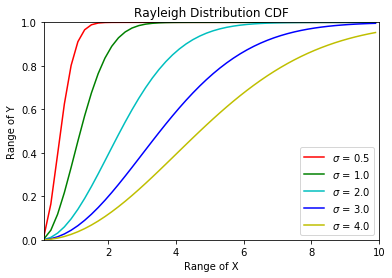
\includegraphics[width=10cm]{Assignment-1/Codes/Figures/CDF.png}
    \caption*{Fig 1.1: Cumulative distribution function}
\end{figure}

\begin{figure}[h!]
    \centering
    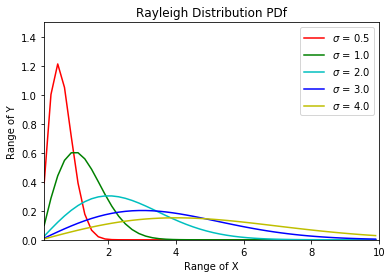
\includegraphics[width=10cm]{Assignment-1/Codes/Figures/PDf.png}
    \caption*{Fig 1.2: Probability density function}
\end{figure}

\subsection*{\boldsymbol{Problem\ 6.1.4}}
Find an expression for $F_A(x)$ using the definition. Plot this expression and compare with the result of problem 6.1.3
\subsection*{\boldsymbol{Solution}}\\
Given,
\begin{align}
A = \sqrt{V}
\end{align}

\begin{align} F_A(x) = P\ (\ A\ \leq\ x)\end{align}
\begin{align} F_A(x) = P\ (\ \sqrt{V}\ \leq\ x)\end{align}
\begin{align} F_A(x) = P\ (\ V\ \leq\ x^2)\end{align}
\begin{align} F_A(x) = F_V(x^2)\end{align}
From (6.1.2.1) we get\\

F_V(x)\ =\ \Bigg\{ 1\ -\ e^{-\alpha x}\ \ \ \ \ ;\ x \geq 0\\

Now\ for\ x^2,\ we\ substitute\ x^2\ in\ place\ of\ x\\

\begin{align}F_V(x^2) = \ \Bigg\{ 1\ -\ e^{-\alpha x^2}\ \ \ \ \ ;\ x^2 \geq 0\end{align}\\


\begin{align*}Putting\ \alpha\ =\ \dfrac{1}{2\sigma^2}\ =\ \dfrac{1}{2}\ \ \ [\because \ \sigma^2\ is\ given\ as\ 1]\end{align*}\\
We get,\\
\begin{align} F_V(x^2)\ =\ 1\ -\ e^\frac{-x^2}{2}\ \ \ \ ;\ x^2\ \geq\ 0\end{align}\\

\begin{mdframed}
Thus the CDF is derived as\\
\begin{align*} F_A(x) =  F_V(x^2)\ =\ 1\ -\ e^\frac{-x^2}{2}\ \ \ \ ;\ x^2\ \geq\ 0\end{align*}
The plot of this equation is shown in Fig 1.3.
\end{mdframed}
\begin{figure}[h!]
    \centering
    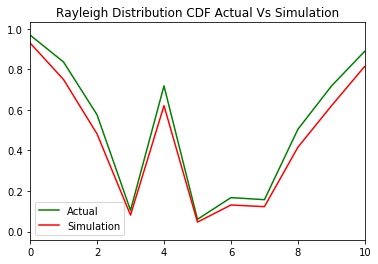
\includegraphics[width=10cm]{Assignment-1/Codes/Figures/cdf_actual_Vs_simulate.png}
    \caption*{Fig 1.3: CDF plot from derived equation}
\end{figure}
\subsection*{\boldsymbol{Problem\ 6.1.5}}
Find an expression for $p_A(x)$ using the definition.

\subsection*{\boldsymbol{Solution}}\\

The PDf can be derived by differentiating the CDF expression from the previous problem 6.1.4
\begin{align}f_A(x) = f_V(x^2)\end{align}
\begin{align}f_V(x^2) = \dfrac{d}{dx}(F_V(x^2))\end{align}
\begin{align}f_V(x^2) = \dfrac{d}{dx}(1 - e^\frac{-x^2}{2})\end{align}
\begin{align}f_V(x^2) = e^\frac{-x^2}{2}.x\end{align}
\begin{mdframed}
\begin{align*}p_A(x) = f_A(x) = e^\frac{-x^2}{2}.x\end{align*}
The plot of this equation is shown in Fig 1.4.
\end{mdframed}
\begin{figure}[h!]
    \centering
    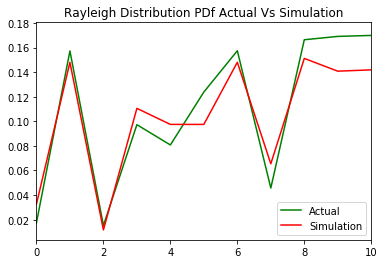
\includegraphics[width=10cm]{Assignment-1/Codes/Figures/pdf_actual_Vs_simulate.png}
    \caption*{Fig 1.4: PDf plot from derived equation}
\end{figure}
\newpage
\text{The theoretical along with simulated PDf and CDF plot of 10,000 samples of two normal random variables}
\newline 
\text{which are further squarred, summed and taken square root of is shown in Fig 1.5 and Fig 1.6 -}

\begin{figure}[h!]
    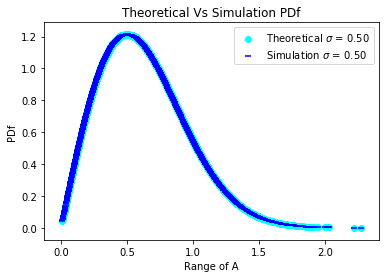
\includegraphics[width=14cm]{Assignment-1/Codes/Figures/theo_Vs_sim_pdf.png}
    \caption*{Fig 1.5: Theoretical Vs Simulation PDf}
\end{figure}
\begin{figure}[h!]
    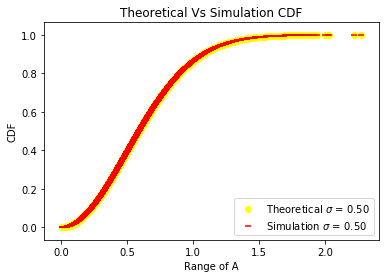
\includegraphics[width=14cm]{Assignment-1/Codes/Figures/theo_Vs_sim_cdf.png}
    \caption*{Fig 1.6: Theoretical Vs Simulation CDF}
\end{figure}
\end{document}
